\begin{frame}
	\myheading{Module 12.3 : Fast RCNN model for object detection}
\end{frame}

%%%%%%%%%%%%%%%%%%%%%%%%%%%%%%%%%%%%%%%%%%%%%%%%%%%%%%%%%%%%%%%%%%%%%%%%%%%%%%%%%%%%%%%%%

\begin{frame}
	\hspace{1cm}
	\begin{columns}
		\column{0.5\textwidth}
		\vspace{0.2cm}
		
		\begin{overlayarea}{\textwidth}{\textheight} 
			\begin{center}
               	\begin{tikzpicture}
	%\node[inner sep=0pt] (A) at (1,4)
	%{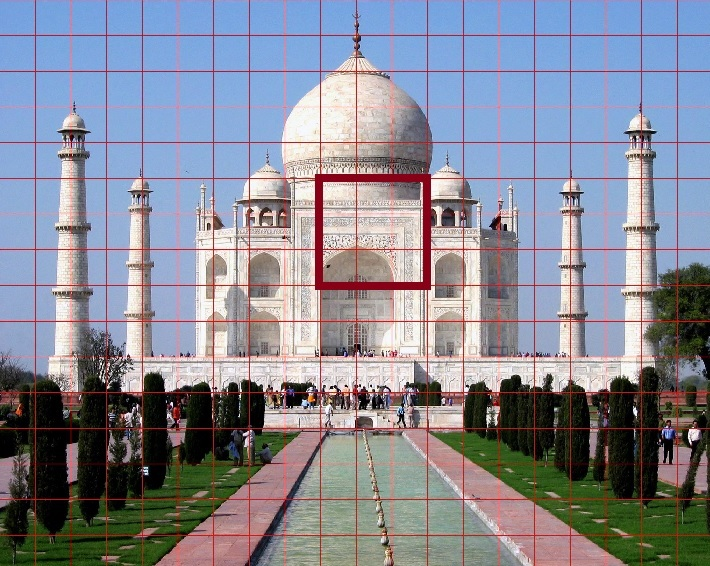
\includegraphics[width=5cm,height=5cm]     {images/CNN}};
	
	\onslide<1->{  \node[inner sep=0pt] (A) at (3,6.5)
		{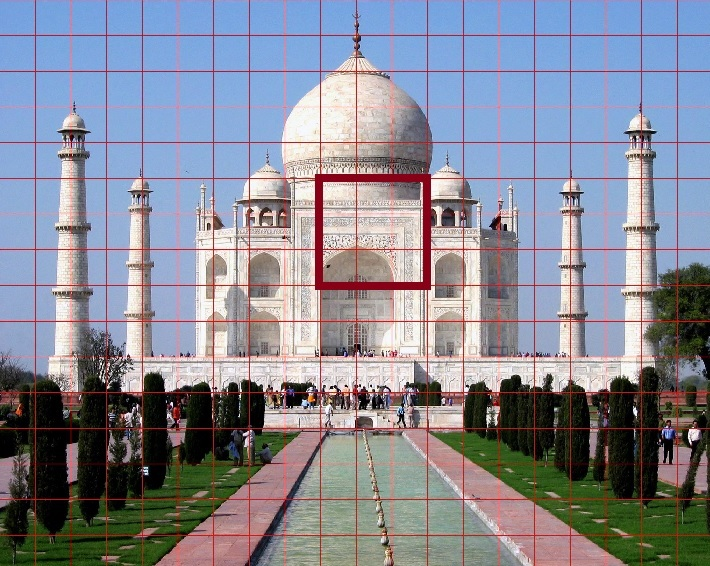
\includegraphics[width=3cm,height=2.2cm]    {images/CNN.jpg}};}
	\onslide<3->{  \node[inner sep=0pt] (A) at (3,4)
		{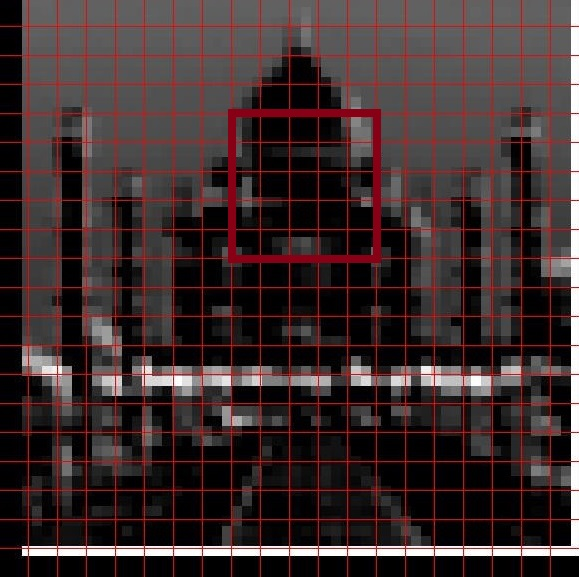
\includegraphics[width=3cm,height=2.2cm]    {images/Conv1_new.jpg}};}
	\onslide<6->{  \node[inner sep=0pt] (A) at (3,1.5)
		{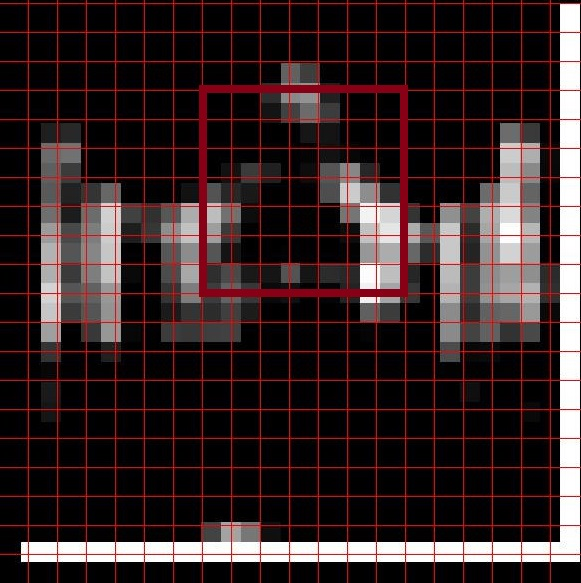
\includegraphics[width=3cm,height=2.2cm]    {images/Conv2_new.jpg}};}
\end{tikzpicture}	
			\end{center}
		\end{overlayarea}   
		\column{0.5\textwidth}
		\vspace{1cm}
		\begin{overlayarea}{\textwidth}{\textheight} 
			\begin{itemize}
				\justifying
				\item<1-> Suppose we apply a $3 \times 3$ kernel on an image
				\item<2-> What is the region of influence of each pixel in the resulting output ?
				\item<3-> Each pixel contributes to a $5 \times 5$ region
				\item<4-> Suppose we again apply a $3 \times 3$ kernel on this output? 
				\item<5-> What is the region of influence of the original pixel from the input ? \onslide<7->{(a $7 \times 7$ region)}
			\end{itemize}
		\end{overlayarea}    
		
	\end{columns}
	
\end{frame}

%%%%%%%%%%%%%%%%%%%%%%%%%%%%%%%%%%%%%%%%%%%%%%%%%%%%%%%%%%%%%%%%%%%%%%%%%%%%%%%%%%%%%%%%%

\begin{frame}
	\noindent
	 \begin{tikzpicture}[scale=0.36]
    
	%\onslide<1->
	{   \renewcommand{\forefillColor}{black!50!white}
		\renewcommand{\borderColor}{white}
		\renewcommand{\toprsidefillcolor}{red}
		%% input layer
		\handmadecube{0}{4.5}{2.5}{-1}{0}
		\renewcommand{\toprsidefillcolor}{green}
                              
		\handmadecube{0}{4.5}{2.5}{-1+0.2}{0}
		\renewcommand{\toprsidefillcolor}{blue!60!white}
                      
		\handmadecube{0}{4.5}{2.5}{-1+0.4}{0}
		\node[scale=0.85] at (1-0.6*2.6-0.1,0-4.8){\tiny{Input}};
		\node [scale=0.7, rotate=53] at (1-0.6*2.6+0.6,0.2) {\tiny{224}};
		\node [scale=0.7, rotate=90] at (1-0.6*2.6+0.2,-2) {\tiny{224}};
      
     
	}
	%% convolution
	%\onslide<2->{ 
	\renewcommand{\forefillColor}{red!50!white}
	\renewcommand{\borderColor}{white}
	\renewcommand{\toprsidefillcolor}{red!50!white!50}
     
	\pgfmathsetmacro{\seedx}{1}
	\pgfmathsetmacro{\seedy}{0}
	\pgfmathsetmacro{\anim}{1}
	\foreach \xct in {1,...,2}
	{
                  
		\pgfmathparse{int(\anim+\xct)}
		%\onslide<\pgfmathresult->
		{
			\pgfmathsetmacro{\xcti}{\seedx+\xct*0.5}
			\pgfmathsetmacro{\ycti}{\seedy}
			\handmadecube{0.5}{4.5}{2.5}{\xcti}{\ycti}
		}
              
              
              
	}
	%\onslide<2->
	{\node[scale=0.85] at (1+0.5,0-4.8){\tiny{Conv}};}
	%\onslide<3->
	{\node [scale=0.7, rotate=53] at (1-0.6*2.6+3.2,0.2) {\tiny{224}};
		\node [scale=0.7, rotate=90] at (1-0.6*2.6+0.2+2.6,-2) {\tiny{224}};
		\node[scale=0.7] at (1+0.725,0-4.2){\tiny{64}};}
	% }
            
	%%%% pooling layer
	%\onslide<4->
	{ 
		\renewcommand{\forefillColor}{blue!50!white}
		\renewcommand{\borderColor}{white}
		\renewcommand{\toprsidefillcolor}{blue!50!white!50}
		\pgfmathsetmacro{\seedx}{3.6}
		\pgfmathsetmacro{\seedy}{0}
                                
		\foreach \xct/\yct in {1}
		{
                       
			\pgfmathsetmacro{\xcti}{\seedx+\xct*0.5}
			\pgfmathsetmacro{\ycti}{\seedy}
			\handmadecube{0.5}{3.8}{1.8}{\xcti}{\ycti}
		}
		\node[scale=0.85] at (1+2.8,0-4.2){\tiny{maxpool}};
		\node [scale=0.6, rotate=53] at (1+3.7,0.2) {\tiny{112}};
		\node [scale=0.6, rotate=90] at (1+3.3,-2+0.5) {\tiny{112}};
		\node[scale=0.7] at (1+2.85,0-3.5){\tiny{64}};
	}  
	%%%% convolution layer
	%\onslide<4->{
	\renewcommand{\forefillColor}{red!50!white}
	\renewcommand{\borderColor}{white}
	\renewcommand{\toprsidefillcolor}{red!50!white!50}
	\pgfmathsetmacro{\seedx}{5.2}
	\pgfmathsetmacro{\seedy}{0}
	\pgfmathsetmacro{\anim}{4}
	\foreach \xct in {1,...,2}
	{
                      
		\pgfmathparse{int(\anim+\xct)}
		%\onslide<\pgfmathresult->
		{
			\pgfmathsetmacro{\xcti}{\seedx+\xct}
			\pgfmathsetmacro{\ycti}{\seedy}
			\handmadecube{0.95}{3.8}{1.8}{\xcti}{\ycti}}
	}  
	%\onslide<5->
	{\node[scale=0.85] at (1+5.25,0-4.2){\tiny{Conv}};}
	%\onslide<6->
	{ \node [scale=0.6, rotate=53] at (1+6.7,0.2) {\tiny{112}};
		\node [scale=0.6, rotate=90] at (1+6.4,-1.5) {\tiny{112}};
		\node[scale=0.6] at (1+5.65,0-3.5){\tiny{128}};}
	%   }      
	%%%%% pooling
	%\onslide<7->
	{       \renewcommand{\forefillColor}{blue!50!white}
		\renewcommand{\borderColor}{white}
		\renewcommand{\toprsidefillcolor}{blue!50!white!50}
		\pgfmathsetmacro{\seedx}{8.8}
		\pgfmathsetmacro{\seedy}{0}
                      
		\foreach \xct/\yct in {1}
		{
			\pgfmathsetmacro{\xcti}{\seedx+\xct*0.5}
			\pgfmathsetmacro{\ycti}{\seedy}
			\handmadecube{0.95}{3.3}{1.3    }{\xcti}{\ycti}
		}  
                  
		\node[scale=0.85] at (1+7.8,0-3.6){\tiny{maxpool}};
		\node [scale=0.6, rotate=49] at (1+8.7,0.1) {\tiny{56}};
		\node [scale=0.6, rotate=90] at (1+8.5,-1.35) {\tiny{56}};
		\node[scale=0.6] at (1+7.8,0-3){\tiny{128}};
                      
	}
	%%%% convolution layer
	%                    \onslide<6->{  
	\renewcommand{\forefillColor}{red!50!white}
	\renewcommand{\borderColor}{white}
	\renewcommand{\toprsidefillcolor}{red!50!white!50}
	\pgfmathsetmacro{\seedx}{10.2}
	\pgfmathsetmacro{\seedy}{0}
	\pgfmathsetmacro{\anim}{7}
	\foreach \xct/\yct in {1,...,3}
	{
		\pgfmathparse{int(\anim+\xct)}
		%\onslide<\pgfmathresult->
		{
			\pgfmathsetmacro{\xcti}{\seedx+1.35*\xct}
			\pgfmathsetmacro{\ycti}{\seedy}
			\handmadecube{1.3}{3.3}{1.3}{\xcti}{\ycti}
		}
	}
                     
	%\onslide<8->
	{  \node[scale=0.85] at (1+11.2,0-3.6){\tiny{Conv}};}
	%\onslide<10->
	{   \node [scale=0.6, rotate=49] at (1+13.625,0.1) {\tiny{56}};
		\node [scale=0.6, rotate=90] at (1+13.425,-1.35) {\tiny{56}};
		\node[scale=0.6] at (1+12.6,0-3){\tiny{256}};
	}
	%}  
	%%%%% pooling
	%\onslide<11->
	{   \renewcommand{\forefillColor}{blue!50!white}
		\renewcommand{\borderColor}{white}
		\renewcommand{\toprsidefillcolor}{blue!50!white!50}
		\pgfmathsetmacro{\seedx}{15.1}
		\pgfmathsetmacro{\seedy}{0}
                          
		\foreach \xct/\yct in {1}
		{
			\pgfmathsetmacro{\xcti}{\seedx+\xct*1.35}
			\pgfmathsetmacro{\ycti}{\seedy}
			\handmadecube{1.3}{2.7}{0.8}{\xcti}{\ycti}
		}
                          
		\node[scale=0.85] at (1+14.8,0-3.2){\tiny{maxpool}};
		\node [scale=0.6, rotate=49] at (1+15.7,0) {\tiny{28}};
		\node [scale=0.6, rotate=90] at (1+15.6,-1.2) {\tiny{28}};
		\node[scale=0.6] at (1+14.8,0-2.4){\tiny{256}};
	}  
	%%%%%%%%% Convolution
	%\onslide<8->{
	\renewcommand{\forefillColor}{red!50!white}
	\renewcommand{\borderColor}{white}
	\renewcommand{\toprsidefillcolor}{red!50!white!50}
	\pgfmathsetmacro{\seedx}{17.1}
	\pgfmathsetmacro{\seedy}{0}
	\pgfmathsetmacro{\anim}{11}
	\foreach \xct/\yct in {1,...,3}
	{
		\pgfmathparse{int(\anim+\xct)}
		%\onslide<\pgfmathresult->
		{
                                   
			\pgfmathsetmacro{\xcti}{\seedx+1.8*\xct}
			\pgfmathsetmacro{\ycti}{\seedy}
			\handmadecube{1.8}{2.7}{0.8}{\xcti}{\ycti}}
	}
                         
	%\onslide<12->
	{  \node[scale=0.85] at (1+18.75,0-3.2){\tiny{Conv}};}                            
		%\onslide<14->
		{\node [scale=0.6, rotate=49] at (1+21.7,0) {\tiny{28}};
		\node [scale=0.6, rotate=90] at (1+21.7,-1.1) {\tiny{28}};
		\node[scale=0.6] at (1+20.75,0-2.4){\tiny{512}};}
	% }
	%%%%%%% pooling
	%\onslide<15->
	{\renewcommand{\forefillColor}{blue!50!white}
		\renewcommand{\borderColor}{white}
		\renewcommand{\toprsidefillcolor}{blue!50!white!50}
		\pgfmathsetmacro{\seedx}{23.2}
		\pgfmathsetmacro{\seedy}{0}
                          
		\foreach \xct/\yct in {1}
		{
			\pgfmathsetmacro{\xcti}{\seedx+\xct*1.8}
			\pgfmathsetmacro{\ycti}{\seedy}
			\handmadecube{1.8}{2.4}{0.6}{\xcti}{\ycti}
		}
                          
		\node[scale=0.85] at (1+23.2,0-3.2){\tiny{maxpool}};
		\node [scale=0.55, rotate=45] at (1+24.15,-0.15) {\tiny{14}};
		\node [scale=0.6, rotate=90] at (1+23.7,-1.1) {\tiny{14}};
		\node[scale=0.6] at (1+23,0-2.2){\tiny{512}};
	}
	%%%%%%%%%% convolution
	%\onslide<10->{
	\renewcommand{\forefillColor}{red!50!white}
	\renewcommand{\borderColor}{white}
	\renewcommand{\toprsidefillcolor}{red!50!white!50}
	\pgfmathsetmacro{\seedx}{25.5}
	\pgfmathsetmacro{\seedy}{0}
	\pgfmathsetmacro{\anim}{15}
                             
	\foreach \xct/\yct in {1,...,3}
	{
		\pgfmathparse{int(\anim+\xct)}
		%\onslide<\pgfmathresult->
		{
                                      
			\pgfmathsetmacro{\xcti}{\seedx+1.8*\xct}
			\pgfmathsetmacro{\ycti}{\seedy}
			\handmadecube{1.8}{2.4}{0.6}{\xcti}{\ycti}
		}
	}  
                             
	%\onslide<16->
	{ \node[scale=0.85] at (1+27.5,0-3.2){\tiny{Conv}};}
	%\onslide<18->
	{   \node [scale=0.55, rotate=45] at (1+30.1,-0.1) {\tiny{14}};
		\node [scale=0.6, rotate=90] at (1+29.6,-1.1) {\tiny{14}};
		\node[scale=0.6] at (1+29,0-2.2){\tiny{512}};}
	% }
	%%%%%% pooling
	%\onslide<19->
	{  \renewcommand{\forefillColor}{blue!50!white}
		\renewcommand{\borderColor}{white}
		\renewcommand{\toprsidefillcolor}{blue!50!white!50}
		\pgfmathsetmacro{\seedx}{31.4}
		\pgfmathsetmacro{\seedy}{-0.25}
                                  
		\foreach \xct/\yct in {1}
		{
			\pgfmathsetmacro{\xcti}{\seedx+\xct*1.8}
			\pgfmathsetmacro{\ycti}{\seedy}
			\handmadecube{1.7}{1.5}{0.3}{\xcti}{\ycti}
		}
                                  
		\node[scale=0.85] at (1+31.5,0-3){\tiny{maxpool}};
		\node [scale=0.6, rotate=10] at (1+32.25,-0.42) {\tiny{7}};
		\node [scale=0.6, rotate=90] at (1+32,-1) {\tiny{7}};
		\node[scale=0.6] at (1+31.5,0-1.6){\tiny{512}};
	}
	%%%%% fc
	%\onslide<12->{
	\renewcommand{\forefillColor}{purple!50!white}
	\renewcommand{\borderColor}{white}
	\renewcommand{\toprsidefillcolor}{purple!50!white!50}
	\pgfmathsetmacro{\seedx}{34}
	\pgfmathsetmacro{\seedy}{4.3}
	\pgfmathsetmacro{\anim}{19}
                 
	\foreach \xct/\yct in {1,...,2}
	{
		\pgfmathparse{int(\anim+\xct)}
		%\onslide<\pgfmathresult->
		{
                           
			\pgfmathsetmacro{\xcti}{\seedx+\xct}
			\pgfmathsetmacro{\ycti}{\seedy}
			\handmadecube{0.6}{10}{0.1}{\xcti}{\ycti}
		}
	}  
                 
                 
                 
	%%fc
	%\onslide<20->
	{ \node[scale=0.85] at (1+33.658,0-5){\tiny{fc}};}
	%        \onslide<22->{ \node[scale=0.85] at (1+35.75,0-5){\tiny{fc}};}
	%\onslide<21->
	{ \node[scale=0.85] at (1+34.75,0-5){\tiny{fc}};}
                 
	%\onslide<20->
	{\node [scale=0.7, rotate=0] at (1+33.658,-6) {\tiny{4096}};}
	%         \onslide<22->{\node [scale=0.7, rotate=0] at (1+35.75,-6) {\tiny{4096}};}
	%\onslide<21->
	{\node [scale=0.7, rotate=0] at (1+34.75,-6) {\tiny{4096}};}
	%}
	%%
	%\onslide<23->
	{  \renewcommand{\forefillColor}{white!50!white}
		\renewcommand{\borderColor}{black}
		\renewcommand{\toprsidefillcolor}{white!50!white!50}
		\handmadecube{1}{6.5}{0.01}{39}{2.5}
                      
		% % softmax
                      
		\node[scale=0.85] at (1+37.5,3){\tiny{softmax}};
                      
                      
		\node [scale=0.7, rotate=0] at (1+37.5,-4.5) {\tiny{1000}};}
	%%
	%\onslide<22->
	{\draw[->,black] (36,-0.7) -- (36.5,-0.7);}
	%\onslide<21->
	{  \draw[->,black] (35,-0.7) -- (35.5,-0.7);}
	%% parameters
	%\onslide<26->
	{
		\draw[->,line width=0.25mm,red] (33.6,-0.7) -- (34.2,-0.7);
	}
	%\onslide<27->
	{ \draw[->,line width=0.25mm,red] (35,-0.7) -- (35.5,-0.7);}
	%\onslide<28->
	{\draw[->,line width=0.25mm,red] (36,-0.7) -- (36.5,-0.7);}
                     
	%\onslide<29->
	{\draw[->,line width=0.25mm,red] (37.2,-0.7) -- (37.8,-0.7);}
                     
\end{tikzpicture}      
	       
\end{frame}

%%%%%%%%%%%%%%%%%%%%%%%%%%%%%%%%%%%%%%%%%%%%%%%%%%%%%%%%%%%%%%%%%%%%%%%%%%%%%%%%%%%%%%%%%

\begin{frame}
	\vspace{1cm}
	\begin{columns}
		\column{0.5\textwidth}
		\begin{overlayarea}{\textwidth}{\textheight}
			\begin{figure}[h!]
				\begin{overprint}
					\onslide<1>\centering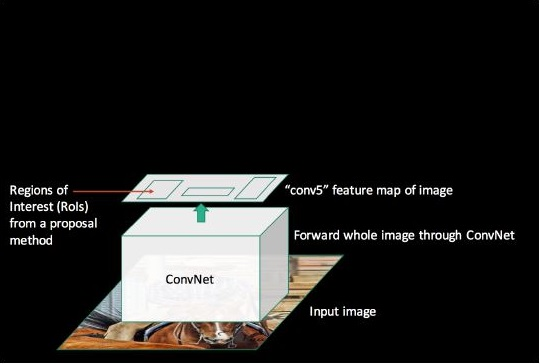
\includegraphics[scale= 0.45]{images/40}\caption[Caption]{\hspace{-90pt} Source: \it{Ross Girshick}}
					\onslide<2>\centering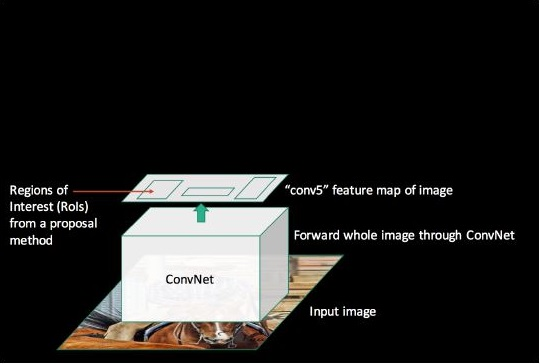
\includegraphics[scale= 0.45]{images/40}\caption[Caption]{\hspace{-90pt} Source: \it{Ross Girshick}}
					\onslide<3>\centering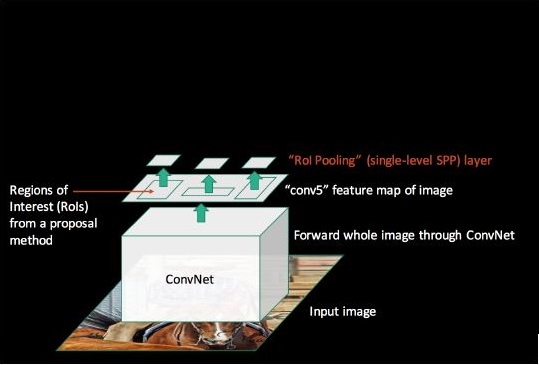
\includegraphics[scale= 0.45]{images/41}\caption[Caption]{\hspace{-90pt} Source: \it{Ross Girshick}}
					\onslide<4->\centering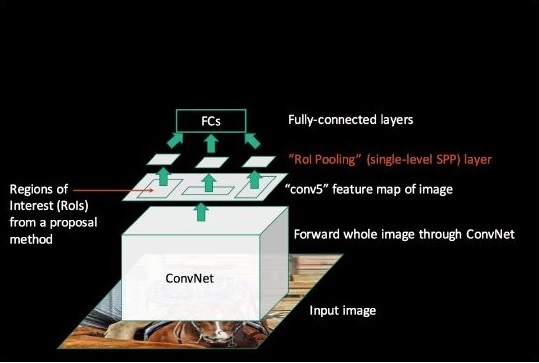
\includegraphics[scale= 0.45]{images/42_fc}\caption[Caption]{\hspace{-90pt} Source: \it{Ross Girshick}}
				\end{overprint} 
			\end{figure}
		\end{overlayarea}     
		\column{0.5\textwidth}
		\begin{overlayarea}{\textwidth}{\textheight}
              
			\begin{itemize}
				\justifying
				\item<1-> Using this idea we could get a bounding box's region of influence on any layer in the CNN 
				\item<2-> The projected Region of Interest (RoI) may be of different sizes
				\item<3-> Divide them into $k$ equally sized regions of dimension $H \times W$ and do max pooling in each of those regions to construct a $k$ dimensional vector 
				\item<4-> Connect the $k$ dimensional vector to a fully connected layer
				\item<5-> This max pooling operation is call RoI pooling 
			\end{itemize}
		\end{overlayarea}
	\end{columns}              
	
\end{frame}

%%%%%%%%%%%%%%%%%%%%%%%%%%%%%%%%%%%%%%%%%%%%%%%%%%%%%%%%%%%%%%%%%%%%%%%%%%%%%%%%%%%%%%%%%

\begin{frame}
	\vspace{1cm}
	\begin{columns}
		\column{0.5\textwidth}
		\begin{overlayarea}{\textwidth}{\textheight}
			\begin{figure}[h!]
				\begin{overprint}
					\onslide<1>\centering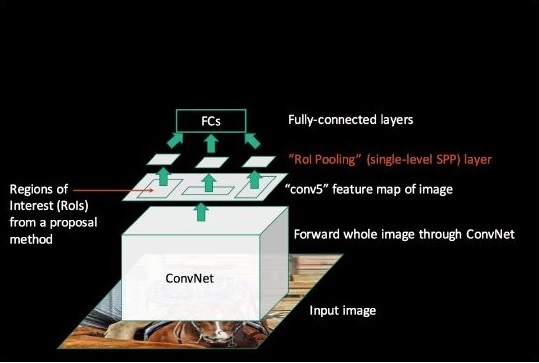
\includegraphics[scale= 0.45]{images/42_fc}\caption[Caption]{\hspace{-90pt} Source: \it{Ross Girshick}}
					\onslide<2>\centering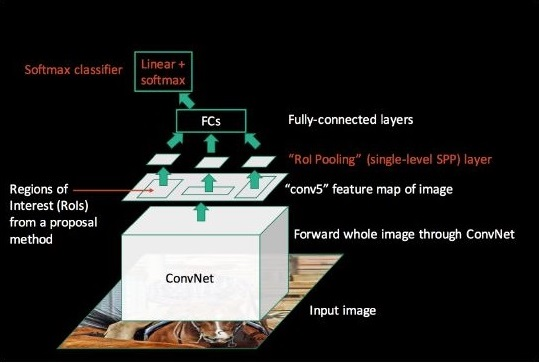
\includegraphics[scale= 0.45]{images/42}\caption[Caption]{\hspace{-90pt} Source: \it{Ross Girshick}}
					\onslide<3>\centering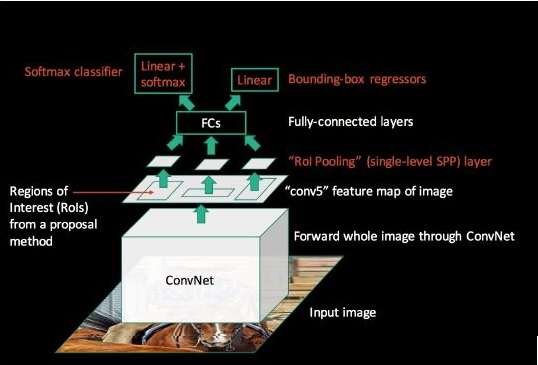
\includegraphics[scale= 0.45]{images/43}\caption[Caption]{\hspace{-90pt} Source: \it{Ross Girshick}}
					\onslide<4->\centering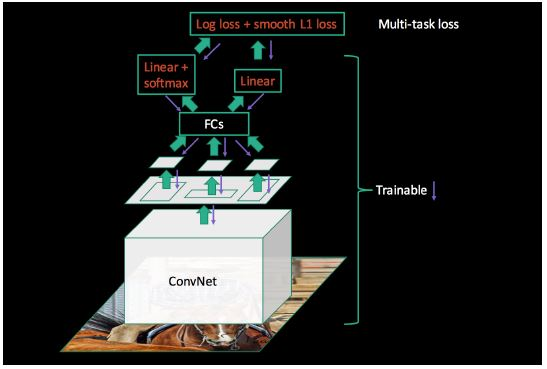
\includegraphics[scale= 0.45]{images/44}\caption[Caption]{\hspace{-90pt} Source: \it{Ross Girshick}}
				\end{overprint} 
			\end{figure}
		\end{overlayarea}     
		\column{0.5\textwidth}
		\begin{overlayarea}{\textwidth}{\textheight}
              
			\begin{itemize}
				\justifying
				\item<1-> Once we have the FC layer it gives us the representation of this region proposal
				\item<2-> We can then add a softmax layer on top of it to compute a probability distribution over the possible object classes
				\item<3-> Similarly we can add a regression layer on top of it to predict the new bounding box $(w^*, h^*, x^*, y^*)$
			\end{itemize}
		\end{overlayarea}
	\end{columns}              
	
\end{frame}

%%%%%%%%%%%%%%%%%%%%%%%%%%%%%%%%%%%%%%%%%%%%%%%%%%%%%%%%%%%%%%%%%%%%%%%%%%%%%%%%%%%%%%%%%

\begin{frame}
	\noindent
	\begin{columns}
		\column{0.5\textwidth}
		\begin{overlayarea}{\textwidth}{\textheight}
			\begin{tikzpicture}[scale=0.4,rotate=90]
	\vspace*{0.1\textwidth}
	\centering    
	\onslide<1->{
		\renewcommand{\forefillColor}{black!50!white}
		\renewcommand{\borderColor}{white}
		\renewcommand{\toprsidefillcolor}{red}

		%% input layer
		\handmadecube{0}{4.5}{2.5}{-1}{0}
		\renewcommand{\toprsidefillcolor}{green}                  
		\handmadecube{0}{4.5}{2.5}{-1+0.2}{0}
		\renewcommand{\toprsidefillcolor}{blue!60!white}          
		\handmadecube{0}{4.5}{2.5}{-1+0.4}{0}
		\node[scale=0.85] at (1-0.6*2.6-0.1,0-4.8-0.5){\tiny{Input}};
		%     \node [scale=0.7, rotate=45] at (1-0.6*2.6+0.6,0.2) {\tiny{224}};
		%     \node [scale=0.7, rotate=90] at (1-0.6*2.6+0.2,-2) {\tiny{224}};


		% Convolution Layer
		\renewcommand{\forefillColor}{red!50!white}
		\renewcommand{\borderColor}{white}
		\renewcommand{\toprsidefillcolor}{red!50!white!50}

		\pgfmathsetmacro{\seedx}{1}
		\pgfmathsetmacro{\seedy}{0}

		\foreach \xct/\yct in {1,...,2}
		{
			\pgfmathsetmacro{\xcti}{\seedx+\xct*0.1}
			\pgfmathsetmacro{\ycti}{\seedy}
			\handmadecube{0.5}{4.5}{2.5}{\xcti}{\ycti}
		}
		\node[scale=0.85] at (1+0.5,0-4.8){\tiny{Conv}};
		%     \node [scale=0.7, rotate=45] at (1-0.6*2.6+3.2,0.2) {\tiny{224}};
		%     \node [scale=0.7, rotate=90] at (1-0.6*2.6+0.2+2.6,-2) {\tiny{224}};
		%     \node[scale=0.7] at (1+0.725,0-4.2){\tiny{64}};
		
		
		
		% Pooling Layer
		\renewcommand{\forefillColor}{blue!50!white}
		\renewcommand{\borderColor}{white}
		\renewcommand{\toprsidefillcolor}{blue!50!white!50}
		
		\pgfmathsetmacro{\seedx}{2.5}
		\pgfmathsetmacro{\seedy}{0}

		\foreach \xct/\yct in {1}
		{
			%       \pgfmathsetmacro{\xcti}{\seedx+\xct*0.1}
			%       \pgfmathsetmacro{\ycti}{\seedy}
			
			\pgfmathsetmacro{\xcti}{\seedx+\xct*0.1}
			\pgfmathsetmacro{\ycti}{\seedy}
			\handmadecube{0.5}{3.8}{1.8}{\xcti}{\ycti}
		}
		\node[scale=0.85] at (0.5+2.8,0-4.2){\tiny{Max-pool}};
		%     \node [scale=0.6, rotate=45] at (1+3.7,0.2) {\tiny{112}};
		%     \node [scale=0.6, rotate=90] at (1+3.3,-2+0.5) {\tiny{112}};
		%     \node[scale=0.7] at (1+2.85,0-3.5){\tiny{64}};
		
		\foreach \xct in {1,2,3}
		{
			\filldraw[fill=gray!60](3+\xct,-1) circle(2pt) ;
		}

		%     \def\yShift{7};
		%     \def\xShift{0};           
		%     \draw (\yShift+0,\xShift+0) rectangle(\yShift+1,\xShift+5);
		
	}
	
	%-----------------------------Slide 1 End ------------------------------------------
	
	
	\onslide<2->{
		\parallelogram{0}{5}{2}{7}{1}
		\node(label) at (7.5,-5) {\tiny{ROI}};  
	}
	
	\onslide<3->{

		%Grid inside Parallelogram          
		\parallelogramWithGrid{0}{5}{2}{7}{1} 

	}
	
	
	\onslide<6->{
		\draw (8.2,-2.2)--(10,-5.5);
		\draw (8.2,2.8)--(10,5.5);
		\draw (10,-5.5) rectangle (11,5.5);
	}     
	
	\onslide<6-7>{
		\node (V_T) at (9.2,-0.5) {
			\begin{footnotesize}
				$W$
			\end{footnotesize}
		};      
	}

	\if 0
	\onslide<8->{
		\draw (13,-5.5) rectangle (14,5.5);
	}
	
	\onslide<8->{
		\node (V_T) at (9.2,-0.5) {
			\begin{footnotesize}
				$V^T$
			\end{footnotesize}
		};      
	}
	
	
	\onslide<8->{
		\node (V_T) at (12.2,-0.5) {
			\begin{footnotesize}
				$U \Sigma$
			\end{footnotesize}
		};
		%\draw (16,-5.5) rectangle (17,5.5);
	}
	
	
		\onslide<8->{
			\node (V_T) at (15.2,-0.5) {
				\begin{footnotesize}
					$U \Sigma$
				\end{footnotesize}
			};      
		}
	\fi           

	%     \filldraw[fill=red](10,3)circle(3pt);

\end{tikzpicture}

		\end{overlayarea}
		
		\column{0.5\textwidth}  
		\begin{overlayarea}{\textwidth}{\textheight}
			\only<1-5>{
				\begin{itemize}
					\justifying
					\item<1-5> Recall that the last pooling layer of VGGNet-16 results in an output of size $512 \times 7 \times 7$ 
					\item<2-5> We replace the last max pooling layer by a RoI pooling layer
					\item<3-5> We set $H=W=7$ and divide each of these RoIs into ($k=49$) regions
					\item<4-5> We do this for every feature map resulting in an ouput of size $512 \times 49$ 
					\item<5-> This output is of the same size as the output of the original max pooling layer
				\end{itemize}
			}
			\only<6->{
				\begin{itemize}
					\justifying
					\item<6-> It is thus compatible with the dimensions of the weight matrix connecting the original pooling layer to the first FC layer
					\item<7-> We can just retain that weight matrix and fine tune it
					%\item<8->  Further speed up can be obtained by replacing $W$ by its truncated SVD $U \Sigma V^T$
				\end{itemize}
			}

			
		\end{overlayarea}
	\end{columns}     
	
\end{frame}

%%%%%%%%%%%%%%%%%%%%%%%%%%%%%%%%%%%%%%%%%%%%%%%%%%%%%%%%%%%%%%%%%%%%%%%%%%%%%%%%%%%%%%%%%

\begin{frame}
	\begin{columns}
		\column{0.5\textwidth}
		\begin{overlayarea}{\textwidth}{\textheight}
			\tikzstyle{input_neuron}=[circle,draw=red!50,fill=red!10,thick,minimum size=4mm]
\tikzstyle{hidden_neuron}=[circle,draw=blue!50,fill=cyan!10,thick,minimum size=4mm]
\tikzstyle{output_neuron}=[circle,draw=green!50,fill=green!10,thick,minimum size=4mm]
\tikzstyle{cpy_neuron}=[circle,draw=red!50,fill=red!50,thick,minimum size=4mm]
\tikzstyle{input}=[circle,draw=black!50,fill=black!20,thick,minimum size=4mm]

\begin{tikzpicture}[scale=0.5, transform shape]
	
	\onslide<1->{
		\node [text width = 30mm] at (2.5,3){Region proposals};
		\node[inner sep=0pt] (A) at (2.5,1.8)
		{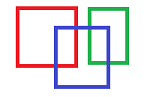
\includegraphics[scale = 0.9]{images/bboxes.png}};

		\node [text width = 34mm] at (6.5,3){Feature extraction};
		\node[inner sep=0pt] (A) at (6.5,2)
		{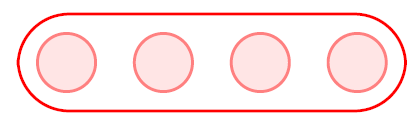
\includegraphics[scale = 0.5]{images/feature.PNG}};
		
		\node [text width = 25mm] at (11.5,3){Classifier};
		\node[inner sep=0pt] (A) at (11.0,2)
		{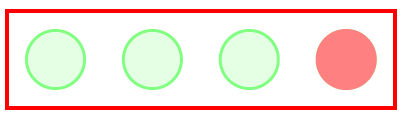
\includegraphics[scale = 0.5]{images/classification.PNG}};
	}
	
	\onslide<1->{
		\node [text width = 25mm] at (0,0){Pre 2012};
		\node[inner sep=0pt] (A) at (2.5,0.2)
		{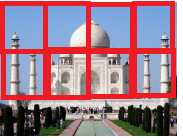
\includegraphics[scale = 0.6]{images/pre_2012.png}};
		\node[inner sep=0pt] (B) at (5.9,0.2)
		{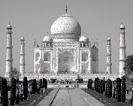
\includegraphics[scale = 0.8]{images/sift.PNG}};
		\node[inner sep=0pt] (C) at (8,0.2)
		{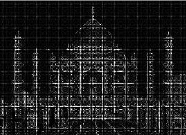
\includegraphics[scale = 0.6]{images/hog.PNG}};
		\node[inner sep=0pt] (D) at (11,0.4)
		{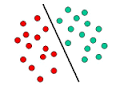
\includegraphics[scale = 0.45]{images/svm.PNG}};
	}
	

	\onslide<1->{
		\node [text width = 25mm] at (0,-1.5){RCNN};
		\node[inner sep=0pt] (A) at (2.5,-1.3)
		{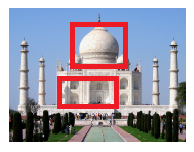
\includegraphics[scale = 0.6]{images/rcnn_bbox.png}};
		\node[inner sep=0pt] (B) at (6.8,-1.4)
		{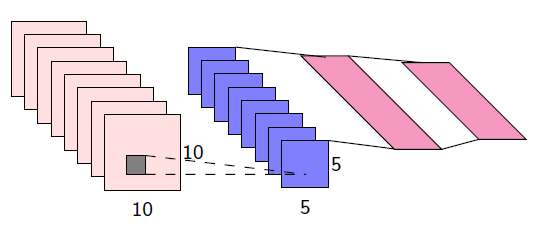
\includegraphics[scale = 0.4]{images/cnn.PNG}};
		\node[inner sep=0pt] (D) at (11,-1.2)
		{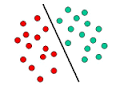
\includegraphics[scale = 0.45]{images/svm.PNG}};
	}
	
	\onslide<1->{
		\node [text width = 25mm] at (0,-3){
		Fast RCNN};
		\onslide<1->{\node[inner sep=0pt] (A) at (2.5,-2.8)
			{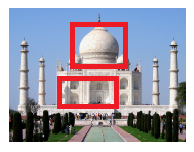
\includegraphics[scale = 0.6]{images/rcnn_bbox.png}};}
		\onslide<2->{\node[inner sep=0pt] (B) at (8.8,-2.9)
			{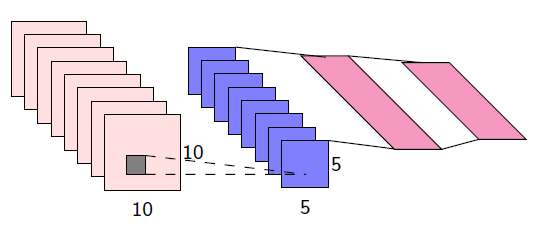
\includegraphics[height=1.5cm,width=6cm]{images/cnn.PNG}};}
		%\onslide<3->{\node[inner sep=0pt] (D) at (11,-2.8)
		%	{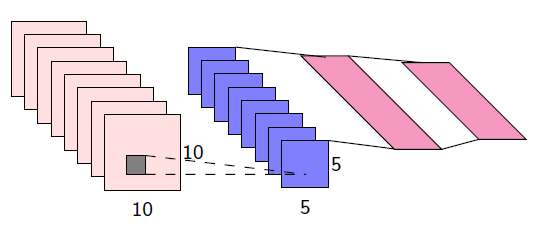
\includegraphics[scale = 0.4]{images/cnn.PNG}};}
	}
	
\end{tikzpicture}

		\end{overlayarea}
		\column{0.5\textwidth}
		\begin{overlayarea}{\textwidth}{\textheight}
			\begin{itemize}
				\justifying
				\item<1-> \textbf{Region Proposals:} Selective Search
				\item<2-> \textbf{Feature Extraction:} CNN
				\item<3-> \textbf{Classifier:} CNN
			\end{itemize}
		\end{overlayarea}
	\end{columns}
\end{frame}
